\documentclass{report}
\usepackage[a4paper,margin=1in]{geometry}
\usepackage{fancyhdr}
\usepackage[titles]{tocloft}
\usepackage{tikz}

\usepackage{multicol}
\usepackage{amsmath}
\usepackage{amssymb}
\usepackage{pdfpages}

%hyperref should be last apparently
\usepackage{hyperref}

\renewcommand\cftsecdotsep{\cftdot}
\renewcommand\cftsubsecdotsep{\cftdot}

\newcommand{\tbf}{\textbf}

\newcommand*{\newpar}{\par\vspace{\baselineskip}\noindent} %start new unindented paragraph with empty line inbetween

\pagestyle{fancy} %allows headers

\lhead{Emma Bach}
\rhead{\today}

\renewcommand*\contentsname{Table of contents}


\begin{document}
\begin{titlepage}
	\centering
	{\Large \textsc{Study Notes}\par}
	\vspace{0.5cm}
	{\huge\bfseries Handbook of Logic in Computer Science\par}
    \vspace{1cm}
	{\Large\itshape Emma Bach\par}

% Bottom of the page
	{\large \today\par}
\end{titlepage}

\tableofcontents
\thispagestyle{fancy}
\chapter{Introduction}
\thispagestyle{fancy}
\section{Definition}
There is no fully rigorous 'mathematical' definition that cleanly seperates everything that is an embedded system from everything that isn't. Instead, embedded systems exist on a spectrum. We can say that a system is \textit{more embedded} or \textit{less embedded} depending on how many of the typical properties of an embedded system apply to it. \tbf{Embedded Systems} are \tbf{computer systems} that tend to:
\begin{itemize}
    \item be \tbf{integrated (embedded) into a larger system}, which they may control and/or provide information processing for.
    \item be \tbf{specialized} to provide exactly the functions they need to.
    \item be forced to work with \tbf{constraints} in time, memory, energy consumption, space, etc.
\end{itemize}
The term \tbf{Cyber-Physical System} generally refers to a larger system that combines computational elements with physical elements, with embedded systems generally being smaller components of such a system.
Examples of Cyber-Physical Systems include \tbf{IoT} (Internet of Things) devices, \tbf{Ubiquitous Computing} devices, and \tbf{SCADA} (Supervisory Control and Data Acquisition) systems.
\newpar
An embedded system generally consists of physical components such as sensors and actuators, computational components including memory and processors, and software. Since the computational components tend to work with digital representation of numbers, while the physical components work with analog voltages, additional conversion through A/D and D/A converters is needed.

\begin{figure}[h!]
\centering

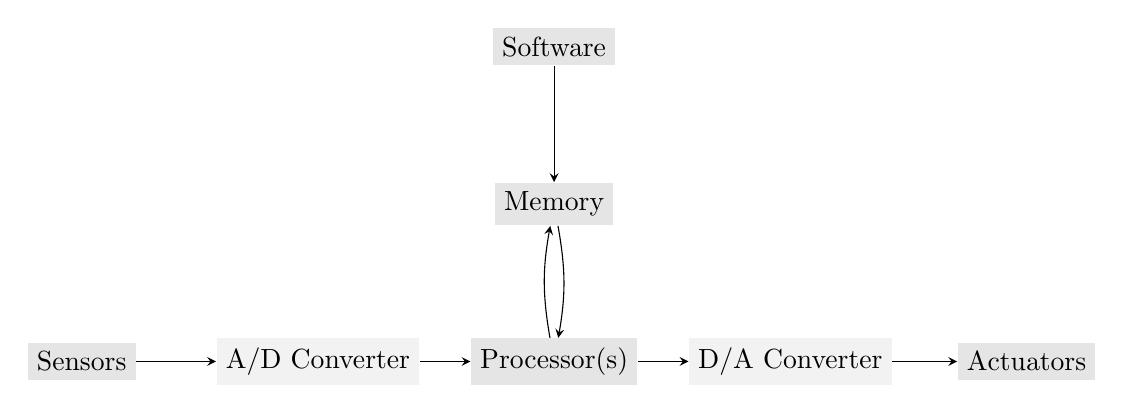
\begin{tikzpicture}[scale=1,-stealth]
\draw[fill=white!90!black] (0,0) node[fill](SE) {Sensors};

\draw[fill=white!95!black] (3,0) node[fill](AD) {A/D Converter};

\draw[fill=white!90!black] (6,0) node[fill](PR) {Processor(s)};
\draw[fill=white!90!black] (6,2) node[fill](ME) {Memory};
\draw[fill=white!90!black] (6,4) node[fill](SO) {Software};

\draw[fill=white!95!black] (9,0) node[fill](DA) {D/A Converter};

\draw[fill=white!90!black] (12,0) node[fill](AC) {Actuators};

\draw (SE) to (AD);
\draw (AD) to (PR);
\draw (SO) to (ME);
\draw (PR) to[bend left=10] (ME);
\draw (ME) to[bend left=10] (PR);
\draw (PR) to (DA);
\draw (DA) to (AC);

\end{tikzpicture}
\caption{The structure of a typical embedded system.}
\label{fig:embeddedsystemstructure}
\end{figure}

\newpar
Embedded systems have extremely widespread applications, especially in fields such as automotive and aerospace engineering and in medical technology.

\section{Design}
Embedded systems must be \tbf{dependable}:
\begin{itemize}
    \item The \tbf{Availability} is the probability of the system working at time t.
    \item The \tbf{Reliability} of an embedded system is the probability of the system working correctly provided that it was working at time t=0.
    \item The \tbf{Maintainability} is the probability of the system working correctly at time t+d after encountering an error at time t.
    \item Additional factors are \tbf{Safety} (How much harm could the system potentially cause?) and \tbf{Security} (How resistant to outside interference is the system?)
\end{itemize}
Since embedded systems are often employed in safety-critical roles, such as in the aforementioned aerospace industry, dependability is extremely important. For safety-critical systems, \tbf{redundancy} is generally a desired trait, so that if one component fails there are still other components to cover the same function.
\newpar
Embedded systems also generally need to be efficient enough to meet constraints in:
\begin{multicols}{2}
\begin{itemize}
    \item Energy consumption
    \item Physical Size
    \item Code Size
    \item Required Memory
    \item Runtime
    \item Weight
    \item Cost
    \item[\vspace{\fill}]
\end{itemize}
\end{multicols}
\newpar
Lastly, Embedded systems are typically \tbf{reactive systems}, meaning that they work through interacting with their environment at a pace dictated by that environment. This often also makes them \tbf{real-time systems}, meaning they need to meet real-time constraints - If a right answer arrives too late, it is just as bad as a wrong answer. If failure to meet a deadline results in catastrophe, that constrained is called a \tbf{hard constraint}. This means that worse average runtimes are acceptable, or even necessary, if it leads to a better worst case runtime. 
\chapter{Specification}
\thispagestyle{fancy}
Design by Contract (\tbf{DbC}), also known as contract programming or simply as internal testing, is the idea that software designers should define precise, formal, verifiable specifications for the desired behaviour of their systems. These often extend the ordinary usage of abstract data types with the description of desired preconditions, postconditions and invariants. Testing can prove the presence of errors, but in order to prove the absence of errors, more complicated methods of Program and Hardware Verification are needed, which are not covered in this course.
\newpar
Such specifications generally involve the \tbf{abstraction} of a given system in order to simplify its description, and hierarchical separation of the description, in order to make a description more easily digestible. We distinguish between two kinds of hierarchy:
\begin{itemize}
    \item Behavioral hierarchy, which describes a systems behavior in terms of states, events, and output signals. Examples of concepts of "high level" behavioral hierarchy are interrupts and exceptions.
    \item Structural hierarchy, which describes how a system can be thought of as a collection of seperate components: processors, actuators, sensors, etc.
\end{itemize}
Specifications generally need to describe a systems \tbf{Timing Behavior}, especially in the case of real-time systems. This involves specifying the elapsed time during execution of a given task, the delay between processes, Timeouts (maximum waiting times for a given event), and Deadlines.
\newpar
It is helpful to model a system as a flow of states (\tbf{State-Oriented Behavior}). However, classical automata are often insufficient, since they don't model timing and don't support hierarchical description.
\section{VHDL}
VHDL is a \tbf{Hardware Description Language}, meaning that it describes digital circuits (instead of abstract algorithms).
\newpar
VHDL code is split into \tbf{entities} and \tbf{architectures}. Entities describe ports, such as inputs (\textit{in}), outputs (\textit{out}), bi-directional ports (\textit{inout}), and \textit{buffers} (Output that the entity itself can read). An architecture defines the actual implementation of an entity - internal wiring, connection of signals, and assignment of values. For example, an OR gate could be implemented as:
\begin{verbatim}
entity orGate is
    port(a,b: in bit;
    c: out bit);
end orGate;
architecture arch1 of orGate is
begin
    c <= a or b;
end arch1;
\end{verbatim}
or:
\begin{verbatim}
entity orGate is
    port(a,b: in bit;
    c: out bit);
end orGate;
architecture arch2 of orGate is
begin
    c <= 1 when (a = '1' or b = '1') else 0;
end arch2;
\end{verbatim}
\newpar
There may be several architectures for a single entity. By default, the most recently analyzed architecture is the one that ends up being used.
\subsection{Testbenches}
A testbench is a VHDL Design without inputs or outputs, designed to test another VHDL Design, generally through Port mapping and verifying that the entity produces the correct outputs for given inputs. For example, a test bench for our OR gate could be realized as:
\begin{verbatim}
entity testbench is
 --empty
end testbench;

architecture test of testbench is
 signal d,e,f: bit := '0'

begin
 or1: entity orGate port map (a=>d,b=>e,c=>f);
 d <= not d after 10 ns;
end;
\end{verbatim}
The \tbf{port map} maps the signals $d,e,f$ in the software to the ports $a,b,c$ in the hardware. It is also possible to use positional association instead of explicit association, which means simply writing
\begin{verbatim}
architecture test of testbench is
 signal d,e,f: bit := '0'

begin
 or1: entity orGate port map (d,e,f);
 d <= not d after 10 ns;
end;
\end{verbatim}
after which the compiler will assign the ports based on the order of the signals in the port map. It is however good practice to always use explicit association.
\newpar
There are three concepts used in  testing:
\begin{itemize}
 \item \texttt{report}, for print-like outputs
 \item \texttt{assert}, for specifying conditions
 \item \texttt{severity}, for specifying how the statement should affect the run of a simulation
\end{itemize}
If needed, combinations of the three can be used within a single line:
\begin{verbatim}
report <message_string>
report <message_string> severity <severity_level>;

assert <condition>;
assert <condition> severity <severity_level>;
assert <condition> report <message_string>;
assert <condition> report <message_string> severity <severity_level>;
\end{verbatim}
If all three are used, the following happens: If the assertion is violated, the program sends a message \texttt{"message"}, and the whole thing is treated as an 'incident' with a predefined \texttt{severity\_level}. If an \texttt{assert} doesn't have a \texttt{severity\_level}, then the severity level will be \texttt{error}. If no \texttt{message\_string} is specified, the message will be \texttt{"Assertion Violation"}.
 If a \texttt{report} without an assertion does not have a \texttt{severity\_level}, the severity level is implicitly defined to be \texttt{note}.
 \newpar
 \texttt{report} statements are inherently sequential, meaning they can occur inside processes, but not (by themselves) in architectures. However, \texttt{assert}ions can be either sequential or concurrent.


\subsection{A Full Adder in VHDL}
\begin{verbatim}
entity fullAdder is

 port(a,b,cin: in bit;
      sum,cout: out bit);

end fullAdder;
\end{verbatim}
Dataflow description of the architecture:
\begin{verbatim}
architecture dataflow of fullAdder is

begin
 sum <= (a xor b) xor cin;
 cout <= (a and b) or (a and cin) or (b and cin);
end dataflow;
\end{verbatim}
\newpar
\tbf{Components} are entities used within a \tbf{structural definition} of an architecture, where a new architecture is defined as an interconnected circuit of already known smaller components. They are defined either via component and signal binding or via entity instantiation. For example, a fully structural definition of a full adder would be something like:
\begin{verbatim}
entity FULLADDER is
  port (A,B, CARRY_IN : in bit;
        SUM, CARRY    : out bit);
end FULLADDER;
 
architecture STRUCT of FULLADDER is
  component HALFADDER
    port (A, B       : in  bit;
          SUM, CARRY : out bit);
  end component;
 
  component ORGATE
    port (A, B : in  bit;
          RES  : out bit);
  end component;
  signal W_SUM, W_CARRY1, W_CARRY2 : bit;
 
begin
 
  MODULE1 : HALFADDER
    port map(A, B, W_SUM, W_CARRY1);
 
  MODULE2 : HALFADDER
    port map (W_SUM, CARRY_IN,
              SUM, W_CARRY2);
 
  MODULE3 : ORGATE
    port map (W_CARRY2, W_CARRY1, CARRY);
 
end STRUCT;
\end{verbatim}
\subsection{Data Types in VHDL}
\subsubsection{Standard data types}
The standard data types provided by VHDL are:
\newpar
\begin{tabular}{|c|c|}
    \hline
    bit & 0,1\\\hline
    boolean & true,false\\\hline
    character & most ASCII characters\\\hline
    integer & $-2^{31} - 1, \ldots, 2^{31}-1$\\\hline
    real & $-1.7e38, \ldots, 1.7e48$\\\hline
    time & 1fs, \ldots, 1hr\\\hline
\end{tabular}
\newpar
Users can also define their own datatypes, either as integer types:
\begin{verbatim}
 --64 bits
type small is range 0 to 63;

 --32 bits
type result32 is range 31 downto 0;

 --16 bits
subtype result16 is result32 range 15 downto 0;
\end{verbatim}
or as enumeration types:
\begin{verbatim}
type state is (idle,start,stop);
type hexDigits is (’0’, {…} , ’9’, ’A’, ’B’, ’C’, ’D’, ’E’, ’F’)
\end{verbatim}
\newpar
It is important not to get confused between statements like the following:
\begin{itemize}
 \item \texttt{signal S : integer range 0 to 3;}, meaning a number between 0 and 3
 \item \texttt{signal S : unsigned(3 downto 0);}, meaning an unsigned 3-bit integer (i.e. a number between 0 and 7)
\end{itemize}
Also note that for most datatypes, \texttt{downto} corresponds to little endian (i.e. most significant bit first), while \texttt{to} corresponds to big endian.

\subsubsection{std\_logic}
In realistic circuits, voltages may come in many forms not accurately described as simple boolean variables / bits. To model these, the datatype \texttt{std\_logic} is used, which contains signal types such as:
\newpar
\begin{tabular}{|c|c|}
    \hline
    0,1 & "Ground" and "High" Voltages\\\hline
    U & uninitialized\\\hline
    X & unknown, impossible to determine (generally a short circuit)\\\hline
    Z & high impedance (circuit connected to neither ground nor voltage)\\\hline
    H & weak drive, logic one (i.e. voltage behind resistor)\\\hline
    L & weak drive, logic zero\\\hline
    W & weak drive, undefined logic value\\\hline 
    - & don't care\\\hline
\end{tabular}
\newpar
These values take priority over each other in the following order: $X > (0 \sim 1) > W > (L \sim H) > Z$.
\newpar
\subsubsection{Arrays and Vectors}
\begin{verbatim}
type intArray is array (15 downto 0) of integer;
type bitArray is array (0 to 7) of bit;
type myMatrix is array (1 to 3, 1 to 3) of std_logic;
subtype myVector4 is std_logic_vector(3 downto 0);
\end{verbatim}
\subsection{Operators}
\newpar
\begin{tabular}{|c|c|c|}
\hline
    No. & Type & Examples\\\hline
    7 & Other Operators & \texttt{abs, not \textrm{(Negation of bits)}, ** \textrm{(exponentiation)}}\\\hline
    6 & Multipliying Operators & \texttt{*, /, mod, rem  \textrm{(remainder)}}\\\hline
    5 & Unary Operators & + (identity), - (negation of a numeric type)\\\hline
    4 & Addition Operators & \texttt{+, -, \&} (vector concatenation)\\\hline
    3 & Shift Operators &\texttt{sll, srl, sla, sra, rol, ror}\footnote[1]{}\\\hline
    2 & Relational Operators & \texttt{=, /= \textrm{(not equal)}, <, <=, >, >=}\\\hline
    1 & Logical Operators &\texttt{and, or, nand, nor, xor, xnor}\\\hline
\end{tabular}
\newpar
$^1$ - Shift operators ending in "l" are "logical", meaning vacated bits are filled with 0. Shift operators ending in "a" are "arithmetical", meaning vacated bits are filled with the value of the rightmost/leftmost bit. The operators "rol" and "ror" rotate the bits instead of shifting them.
\newpar
Operators with higher numbers in this table take priority over operators with lower numbers.
\subsection{Constants and Signals}
Constants work as expected in a programming language:
\begin{verbatim}
constant PI: real := 3.1415;
contant PERIOD: time := 100ns;
type vecType is array (0 to 3) of integer;
contant VEC: vecType := (2,4,-1,7)
\end{verbatim}
Signals represent a wire or register. They can be of any data type, can be declared in architectures only.
\begin{verbatim}
signal sum: std_logic;
signal clk: bit;
signal data: std_logic_vector(0 to 7) := "00X0X011";
signal value: integer range 16 to 31 := 17;
\end{verbatim}
Signals assignments are performed \tbf{concurrently}, meaning that they are sequentially collected until the process is stopped, and then collectively performed in parallel after al processes are stopped.
\newpar
Signals can be assigned with either an explicit user-defined time delay ("after 10ns", etc.), or with an implicit small delta delay:
\begin{verbatim}
sum <= (a xor b) after 2 ns; -- explicit delay
data(1) <= 'x'; -- implicit delay
\end{verbatim}
Signal assignments can also include conditionals. This can be done using the when-else condition:
\begin{verbatim}
clk <= '0' after 5ns when clk = '1' else '1' after 7ns when clk = '0';
a <= "1000" when b = "00" 
else "0100" when b = "01" 
else "0010" when b= "10" 
else "0001" when b = "11";
\end{verbatim}
Or using the with-select condition:
\begin{verbatim}
with b select a <=
	"1000" when "00",
	"0100" when "01",
	"0010" when "10",
	"0001" when "11";
\end{verbatim}
Neither of the two conditionals may be used inside a process. Within the finished hardware, conditions like this are realized using a multiplexer. Custom multiplexer code would look something like this:
\begin{verbatim}
entity mux is
port (i3, i2, i1, i0: in bit;
    sel: in bit_vector(1 downto 0);
    otp: out bit);
end;    

architecture wSelect of mux is
begin
    with sel select
    otp <= i0 when "00",
    i1 when "01",
    i2 when "10",
    i3 when others;
end;
\end{verbatim}
\subsection{Variables}
Variables work like variables in other programming languages. They store temporary values and are only usable in processes, procedures and functions. \tbf{Usage of them is not recommended in VHDL for synthesis.} Unlike signal assignments, variables assignments are performed sequentially as they are encountered in the code.
\subsection{Processes}
We've already seen two styles of modelling using VHDL: A Dataflow architecture uses concurrent signal assignment statements, while a structural architecture uses only component instantiation statements. We will now learn a third style: \tbf{Behavioural architecture}, which uses  \tbf{process statements}. A process is simply a set of statements that are executed sequentially-ish:
\begin{verbatim}
signal clk : std_logic := '0';
clk_gen: process ( )
begin
 clk <= ‘0’;
 wait for 10 ns;
 clk <= ‘1’;
 wait for 10 ns;
end process;
\end{verbatim}
VHDL supports four different types of wait statements:
\begin{itemize}
    \item \texttt{wait on} waits until one of the given signals changes (e.g. \texttt{wait on a,b,c;}).
    \item \texttt{wait until} waits until the given condition is met (e.g. \texttt{wait until (clkEvent and clk = '1')}).
    \item \texttt{wait for} waits for a specified amount of time (e.g. \texttt{wait for 25 ns;}).
    \item \texttt{wait} waits indefinitely.
\end{itemize}
Only simple signal assignments are allowed inside a process. When a simulation starts, each process will be executed at least once. Afterwards, they will loop infinitely. If the process has a \textit{sensitivity list}, a new iteration will occur whenever a signal from the sensitivity list changes:
\begin{verbatim}
entity DFF is
port (D, clk: in std_logic;
Q: out std_logic);
end DFF;
architecture rtl of DFF is
begin
 p : process(clk) -- sensitivity list
 begin
 if (clk‘event) and (clk=`1`) then
  Q <= D;
 end if;
 end process p;
end rtl;    
\end{verbatim}
Processes with sensitivity lists are equivalent to processes without a sensitivity loop that have \texttt{wait on} statements instead:
\begin{verbatim}
entity DFF is
port (D, clk: in std_logic;
Q: out std_logic);
end DFF;
architecture rtl of DFF is
begin
 p : process
 begin
  if (clk‘event) and (clk=`1`) then
   Q <= D;
  end if;
  wait on clk; -- equivalent wait statement
 end process p;
end rtl;
\end{verbatim}
Processes are not allowed to have subprocesses. They always loop, and are often used to specify sequential hardware. Everything in VHDL is implicitly part of a "main" process.
\subsection{Statements}
\texttt{if}-Statements and \texttt{case}-Statements are comparable to \texttt{if}-Statements and \texttt{switch}-statements in other languages. Both of them can be nested. Conditions in \texttt{if}-Statements can be any boolean expression.
\begin{multicols}{2}
\begin{verbatim}
if a = b then
…
elsif a > b or a > c then
…
else
…
end if;    
\end{verbatim}
\begin{verbatim}
case a is
when "01" =>
…
when "10" =>
…
when others =>
null
end case;    
\end{verbatim}
\end{multicols}
\newpar
As seen here, a case where nothing happens can be specified using the \texttt{null} Statement.
\newpar
VHDL also supports \texttt{loop}s. Here are two variants of a clock that counts up to 10, incrementing once every 5ns, using a \texttt{while} loop and a \texttt{for} loop:
\begin{multicols}{2}
\begin{verbatim}
constant MAX_SIM_TIME : time := 50 ns;
constant PERIOD : time := 10 ns;
...
clk_gen: process (clk)
begin
 while NOW < MAX_SIM_TIME loop --!
  clk <= not clk ;
  wait for PERIOD/2;
 end loop;
 wait;
end process clk_gen;
\end{verbatim}
\begin{verbatim}
constant MAX_CYCLES : integer := 10;
constant PERIOD : time := 10 ns;
...
clk_gen: process (clk)
variable cnt: integer := 0
begin
 for cnt in 1 to MAX_CYCLES loop --!
  clk <= not clk ;
  wait for PERIOD/2;
 end loop;
 wait;
end process clk_gen;
\end{verbatim}
\end{multicols}
\newpar
And a third variant using the \texttt{exit when}-Statement:
\begin{verbatim}
constant MAX_CYCLES : integer := 10;
...
clk_gen: process (clk)
variable cnt: integer := 0;
begin
 L1: loop
  clk <= not clk;
  cnt := cnt + 1;
  wait for 5ns;
 exit when cnt > 2*MAX_CYCLES; --!
end loop;
wait;
end process clk_gen;
\end{verbatim}
\newpar
During synthesis, all loops have to be unrolled, meaning that loops with a non-static range are non-synthesisable. It is generally good practice to only use loops in testbenches.
\subsection{Functions and procedures}
Apart from entities and architectures, VHDL also supports functions and procedures, similar to traditional programming languages. A \tbf{Function} has a return value and can be used in statements:
\begin{verbatim}
architecture rtl of example is
 signal test : integer := 0;
 ...

begin
 function b2i(b : bit) return integer is
 begin
  if b = '1' then
   return 1;
  else
   return 0;
  end if;
 end b2i;

 test <= b2i(’0’);
end;
\end{verbatim}
Functions can be overloaded, meaning that there can be Functions with the same name but different type signatures. By default, functions have to be \tbf{pure}, meaning they are free of side effects - formally $f(a)$ always returns the same value if $a$ is the same. An impure function can be declared by prepending the function with \texttt{impure}. This will let the function gain access to all variables and signals outside of its scope.
\newpar
A \tbf{Procedure} can be seen as a function without a return value. Instead, it has \texttt{in, out} or \texttt{inout}-signals, similar to an entity:
\begin{verbatim}
architecture behave of ex_procedure_simple is
 signal r_TEST : std_logic_vector(7 downto 0) := X"42";

-- Purpose: Increments a std_logic_vector by 1
 procedure INCREMENT_SLV (
  signal r_IN : in std_logic_vector(7 downto 0);
  signal r_OUT : out std_logic_vector(7 downto 0)
  ) is
  begin
   r_OUT <= std_logic_vector(unsigned(r_IN) + 1);
  end INCREMENT_SLV;
...
 signal test : std_logic_vector(7 downto 0) := (others => '0');
...
 test_p: process
 begin
  INCREMENT_SLV(test, test);
 end test_p;
\end{verbatim}
Because Procedures do not return anything, they can't be used in statements. They can still be used inside of processes, or, if \texttt{out} and \texttt{inout} parameters are signals, as their own processes.
\subsection{Synthesisable vs Non-Synthesisable Code}
Only a subset of VHDL statements is \tbf{synthesisable} (i.e. compilable with the output being hardware). Non-synthesisable statements include time statements, asserts, and dynamic loops.
\newpar
You can work around many of these restrictions. For example, the following code is non-synthesisable, because it uses a \texttt{wait}-Statement:
\begin{verbatim}
architecture behavior of testbench is
begin
 enable <= '0';
 wait for 100 ns; -- !
 enable <= '1'
end behavior;
\end{verbatim}
However, the following code is synthesisable:
\begin{verbatim}
architecture behavior of realCircuit is
signal cnt : unsigned(3 downto 0) := (others => '0');
begin
 process ( clk )
 begin
  if rising_edge( clk ) then
   if cnt < 10 then -- assume clk  period is 10 ns
    cnt <= cnt + 1;
    enable <= '0';
   else
    cnt <= (others => '0');
    enable <= '1';
   end if;
  end if;
 end process;
end behavior;
\end{verbatim}
\newpar
Many statements in VHDL are technically synthesisable, but are best avoided, generally because they quickly lead to significant, often unexpected, increases in hardware complexity. These include:
\begin{itemize}
 \item division or multiplication with numbers that aren't powers of 2
 \item \texttt{if rising\_edge (clk)} with \texttt{else}
 \item latches
\end{itemize}
\newpar
a \tbf{latch} is a memory element that is triggered by a changes immediately whenever the input changes:
\begin{verbatim}
architecture rtl of latch is
…
begin
 process (E, D) begin
  if E = ’1’ then
   Q <= D;
  end if;
 end process;
end;
\end{verbatim}
The big problem with latches is that they leaf to uncertainty in a circuit's timing behavior. You can avoid latches by including a clock and triggering things only on rising edges, and by stating all possibilities in if statements.
\subsection{Simulation}
A simulation works in the following way:
\begin{itemize}
\item Initialization:
\begin{itemize}
 \item Initialize all signals
 \item Set simulation time to 0
 \item Execute all processes once
 \item Start simulaton cycles
\end{itemize}
\item Simulation cycles:
\begin{itemize}
 \item update signals
 \item execute processes
 \item repeat
\end{itemize}
\item Simulation ends when:
\begin{itemize}
 \item No more signal changes are possible
 \item A maximum simlulation time has been reached
 \item An explicit \texttt{wait} is encountered
\end{itemize}
\end{itemize}
\newpar
Values are assigned to signals using a \tbf{transaction list}. The list contains entries of the form $(s,v,t)$, meaning ``signal $s$ is set to value $v$ at time $t$''. Processes are similarly reactivated using a \tbf{process activation list}, with entries of the form $(p,t)$ (``process $p$ resumes at time $t$'').
\subsection{Delay Modeling}
Real components always work on a delay. \tbf{Delay of components} can be modeled in VHDL using the \texttt{inertial} Keyword:
\begin{verbatim}
output <= not input after 10 ns;
-- with inertial delay:
output <= reject 5 ns inertial not input after 10 ns;
\end{verbatim}
If a signal assignment happens for an amount of time shorter than the signals inertial delay, then the signal doesn't change at all.
\newpar
There is also the Keyword \texttt{transport} to model the \tbf{delay of wires}:
\begin{verbatim}
output <= not input after 10 ns;
-- with transport delay:
output <= transport not input after 10 ns;
\end{verbatim}
A signal that uses \texttt{transport} delay always gets changed after the specified time.
\clearpage
\chapter{Design Space Evaluation}
Design Space Evaluation is the process of considering different possible ways to realize a given plan and comparing them based on criteria such as:
\begin{multicols}{2}
\begin{itemize}
 \item Cost
 \item Performance
 \item Power consumption
 \item Quality
\end{itemize}
\end{multicols}
\newpar
'Cost' can be further split into factors such as:
\begin{multicols}{2}
 \begin{itemize}
  \item Manufacturing cost
  \item Design cost
  \item Field support
  \item Administration
  \item Design time
  \item[\vspace{\fill}]
 \end{itemize}
\end{multicols}
While 'Performance' comes down to factors like:
\begin{multicols}{2}
\begin{itemize}
 \item Clock Frequency / Operations per Second
 \item Bandwidth
 \item Quality of service
 \item[\vspace{\fill}]
\end{itemize}
\end{multicols}
\newpar
Note that especially in safety-critical systems, it is preferable to accept a worse average runtime if it leads to a better worst case runtime and more predictability. For example, caching is usually avoided because of its inherent unpredictability.
\newpar
Within the context of Embedded Systems, common decision points include choosing between:
\begin{multicols}{3}
\begin{itemize}
 \item ASICs (Application specific integrated circuits)
 \item Field Programmable Gate Arrays (FPGAs)
 \item Microprocessors
 \item Microcontrollers
 \item Different Memory Architectures
 \item Different Interfaces (I$^2$C, SPI, CAN, \ldots)
 \item Different possible Sensors \& Actuators
 \item Different possible AD and DA converters
 \item etc.
\end{itemize}
\end{multicols}
\newpar
Formally, this comes down to a \tbf{multiobjective optimisation problem}.
\newpar
Generally, \tbf{power} is the most important constraint in Embedded Systems, and thus minimizing power consumption is one of the primary concerns during the design process.
%
\chapter{Hardware}
\thispagestyle{fancy}
%
\chapter{Software}
\thispagestyle{fancy}
A big software chapter was teased all throughout the lecture but besides a non-exam-relevant chapter on the very very basic basics of embedded AI it was basically skipped :\textsuperscript{$\wedge$})
%
\appendix
\chapter{Sources}
\thispagestyle{fancy}
The content of these notes primarily comes from the slides provided by Prof. Amft and Lars Häusler.
\newpar
Additional sources include \href{http://www.en.wikipedia.org}{Wikipedia} for theoretical topics and \href{http://www.vhdlwhiz.com}{vhdlwhiz.com}, \href{http://www.vhdl-online.de}{vhdl-online.de} and \href{https://www.sigasi.com/tech/}{sigasi.com} for VHDL.
\newpar
A tool of dubious quality that was nevertheless used frequently throughout the lecture for playing around with VHDL was \href{https://www.edaplayground.com}{edaplayground.com}.
\end{document}
